\documentclass{beamer}

 \pdfmapfile{+sansmathaccent.map}


\mode<presentation>
{
  \usetheme{Warsaw} % or try Darmstadt, Madrid, Warsaw, Rochester, CambridgeUS, ...
  \usecolortheme{crane} % or try seahorse, beaver, crane, wolverine, ...
  \usefonttheme{serif}  % or try serif, structurebold, ...
  \setbeamertemplate{navigation symbols}{}
  \setbeamertemplate{caption}[numbered]
} 

\renewcommand{\familydefault}{\rmdefault}


\hypersetup{
    colorlinks=true,
    linkcolor=blue,
    filecolor=blue,      
    urlcolor=blue,
}

\usepackage{amsmath}
\usepackage{mathtools}

\DeclareMathOperator*{\argmin}{arg\,min}

\usepackage{subcaption}

\usepackage{tikz}
\tikzset{every picture/.style={line width=0.75pt}} %set default line width to 0.75pt        
%%%%%%%%%%%%%%%%%%%%%%%%%%%%%%%%%%%%%%%%%%%%%%%%%%%


\usepackage{listings}
\usepackage{color}
\definecolor{mygreen}{rgb}{0,0.6,0}
\definecolor{mygray}{rgb}{0.5,0.5,0.5}
\definecolor{mymauve}{rgb}{0.58,0,0.82}

\definecolor{cof}{RGB}{255,187,0}
\definecolor{pur}{RGB}{205,137,0}
\definecolor{greeo}{RGB}{91,173,69}
\definecolor{greet}{RGB}{52,111,72}

\usetikzlibrary{fadings}
\usetikzlibrary{patterns}
\usetikzlibrary{shadows.blur}
\usetikzlibrary{shapes}

\lstset{ 
  backgroundcolor=\color{white},   % choose the background color; you must add \usepackage{color} or \usepackage{xcolor}; should come as last argument
  basicstyle=\footnotesize,        % the size of the fonts that are used for the code
  breakatwhitespace=false,         % sets if automatic breaks should only happen at whitespace
  breaklines=true,                 % sets automatic line breaking
  captionpos=b,                    % sets the caption-position to bottom
  commentstyle=\color{mygreen},    % comment style
  deletekeywords={...},            % if you want to delete keywords from the given language
  escapeinside={\%*}{*)},          % if you want to add LaTeX within your code
  extendedchars=true,              % lets you use non-ASCII characters; for 8-bits encodings only, does not work with UTF-8
  firstnumber=0000,                % start line enumeration with line 0000
  frame=single,	                   % adds a frame around the code
  keepspaces=true,                 % keeps spaces in text, useful for keeping indentation of code (possibly needs columns=flexible)
  keywordstyle=\color{blue},       % keyword style
  language=Octave,                 % the language of the code
  morekeywords={*,...},            % if you want to add more keywords to the set
  numbers=left,                    % where to put the line-numbers; possible values are (none, left, right)
  numbersep=5pt,                   % how far the line-numbers are from the code
  numberstyle=\tiny\color{mygray}, % the style that is used for the line-numbers
  rulecolor=\color{black},         % if not set, the frame-color may be changed on line-breaks within not-black text (e.g. comments (green here))
  showspaces=false,                % show spaces everywhere adding particular underscores; it overrides 'showstringspaces'
  showstringspaces=false,          % underline spaces within strings only
  showtabs=false,                  % show tabs within strings adding particular underscores
  stepnumber=2,                    % the step between two line-numbers. If it's 1, each line will be numbered
  stringstyle=\color{mymauve},     % string literal style
  tabsize=2,	                   % sets default tabsize to 2 spaces
  title=\lstname                   % show the filename of files included with \lstinputlisting; also try caption instead of title
}




%%%%%%%%%%%%%%%%%%%%%%%%%%%%%%%%%%%%%%%%%%%%%%%%%%%%%


\title{Quadratically constrained quadratic programming, \\ Second-order cone programming }
\subtitle{Computational Intelligence, Lecture 8}
\author{by Sergei Savin}
\centering
\date{Fall 2020}



\begin{document}
\maketitle


\begin{frame}{Content}

\begin{itemize}
\item  Quadratic programming: recap
\item  Quadratically constrained quadratic programming
\begin{itemize}
    \item General form
    \item Domain
\end{itemize}
\item  Second-order cone programming
\begin{itemize}
    \item General form
    \item Special cases
    \item Friction cone
    \item Friction cone, solution
\end{itemize}
\item Homework
\end{itemize}

\end{frame}



\begin{frame}{Quadratic programming}
\framesubtitle{General form}
\begin{flushleft}

Remember the general form of a quadratic program:

%
\begin{equation}
\begin{aligned}
& \underset{\mathbf{x}}{\text{minimize}}
& & \mathbf{x}^\top \mathbf{H} \mathbf{x} + \mathbf{f}^\top\mathbf{x}, \\
& \text{subject to}
& & \begin{cases}
    \mathbf{A}\mathbf{x} \leq \mathbf{b}, \\
    \mathbf{C}\mathbf{x} = \mathbf{d}.
    \end{cases}
\end{aligned}
\end{equation}

where $\mathbf{H}$ is positive-definite and $\mathbf{A}\mathbf{x} \leq \mathbf{b}$ describe a convex region.
 
\end{flushleft}
\end{frame}




\begin{frame}{Quadratically constrained quadratic programming}
\framesubtitle{General form}
\begin{flushleft}

General form of a quadratically constrained quadratic program (QCQP) is given below:

%
\begin{equation}
\begin{aligned}
& \underset{\mathbf{x}}{\text{minimize}}
& & \mathbf{x}^\top \mathbf{P}_0 \mathbf{x} + \mathbf{q}_0^\top\mathbf{x}, \\
& \text{subject to}
& & \begin{cases}
    \mathbf{x}^\top \mathbf{P}_i \mathbf{x} + \mathbf{q}_i^\top\mathbf{x} + r_i \leq 0, \\
    \mathbf{A}\mathbf{x} = \mathbf{b}.
    \end{cases}
\end{aligned}
\end{equation}

where $\mathbf{P}_i$ are positive-definite.
 
\end{flushleft}
\end{frame}



\begin{frame}{Quadratically constrained quadratic programming}
\framesubtitle{Domain}
\begin{flushleft}

Domain of a QCQP without equality constraints and with no degenerate inequality constraints is an intersection of ellipses:

\begin{figure} [h!]
\begin{center}

\tikzset{every picture/.style={line width=0.75pt}} %set default line width to 0.75pt        

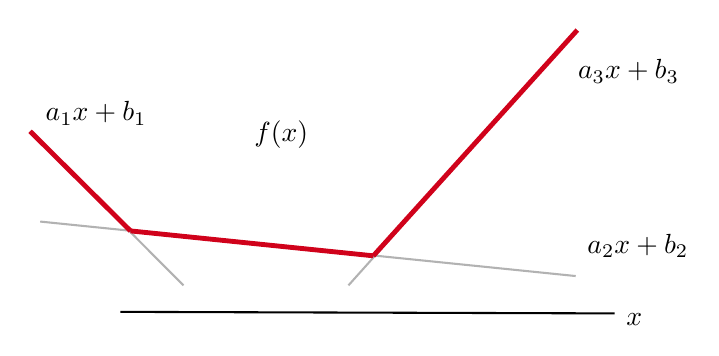
\begin{tikzpicture}[x=0.75pt,y=0.75pt,yscale=-0.75,xscale=0.75]
%uncomment if require: \path (0,300); %set diagram left start at 0, and has height of 300

%Straight Lines [id:da12023127812313228] 
\draw    (158,238) -- (475.5,239) ;
%Straight Lines [id:da35376749976820165] 
\draw  [draw opacity=0.3, line width=0.75pt]  (100,122) -- (198.5,221) ;
%Straight Lines [id:da0760682183068686] 
\draw  [draw opacity=0.3, line width=0.75pt]  (106.5,180) -- (450.5,215) ;
%Straight Lines [id:da032661760394889994] 
\draw  [draw opacity=0.3, line width=0.75pt]  (451.5,57) -- (304.5,221) ;
%Straight Lines [id:da0067101665100168795] 
\draw [color={rgb, 255:red, 208; green, 2; blue, 27 }  ,draw opacity=1, line width=1.75pt]    (320.5,202) -- (164.5,186) ;
%Straight Lines [id:da3516811366133792] 
\draw [color={rgb, 255:red, 208; green, 2; blue, 27 }  ,draw opacity=1, line width=1.75pt]    (100,122) -- (164.5,186) ;
%Straight Lines [id:da5842320764486784] 
\draw [color={rgb, 255:red, 208; green, 2; blue, 27 }  ,draw opacity=1, line width=1.75pt]    (451.5,57) -- (320.5,202) ;

% Text Node
\draw (242,113) node [anchor=north west][inner sep=0.75pt]   [align=left] {$\displaystyle f( x)$};
% Text Node
\draw (108,101) node [anchor=north west][inner sep=0.75pt]   [align=left] {$\displaystyle a_{1} x+b_{1}$};
% Text Node
\draw (456,186) node [anchor=north west][inner sep=0.75pt]   [align=left] {$\displaystyle a_{2} x+b_{2}$};
% Text Node
\draw (450,74) node [anchor=north west][inner sep=0.75pt]   [align=left] {$\displaystyle a_{3} x+b_{3}$};
% Text Node
\draw (481,237) node [anchor=north west][inner sep=0.75pt]   [align=left] {$\displaystyle x$};
\end{tikzpicture}
\end{center} 
% \caption{AR 601 bipedal robot, Innopolis University}
\end{figure}
 
\end{flushleft}
\end{frame}




\begin{frame}{Second-order cone programming}
\framesubtitle{General form}
\begin{flushleft}


The general form of a Second-order cone program (SOCP) is:

%
\begin{equation}
\begin{aligned}
& \underset{\mathbf{x}}{\text{minimize}}
& & \mathbf{f}^\top\mathbf{x}, \\
& \text{subject to}
& & \begin{cases}
    ||\mathbf{A}_i\mathbf{x} + \mathbf{b}_i||_2 \leq 
     \mathbf{c}_i^\top \mathbf{x} + d_i, \\
    \mathbf{F}\mathbf{x} = g.
    \end{cases}
\end{aligned}
\end{equation}

LP, QP and QCQP are subsets of SOCP.
 
\end{flushleft}
\end{frame}



\begin{frame}{Second-order cone programming}
\framesubtitle{Special cases}
\begin{flushleft}

We can write problem where our domain is a ball as SOCP:
%
\begin{equation}
\begin{aligned}
& \underset{\mathbf{x}}{\text{minimize}}
& & \mathbf{f}^\top\mathbf{x}, \\
& \text{subject to}
& & ||\mathbf{x}||_2 \leq d_i
\end{aligned}
\end{equation}

\bigskip

Same for ellipsoidal constraints:
%
\begin{equation}
\begin{aligned}
& \underset{\mathbf{x}}{\text{minimize}}
& & \mathbf{f}^\top\mathbf{x}, \\
& \text{subject to}
& & ||\mathbf{A}_i\mathbf{x}||_2 \leq d_i
\end{aligned}
\end{equation}
 
\end{flushleft}
\end{frame}



\begin{frame}{Second-order cone programming}
\framesubtitle{Friction cone}
\begin{flushleft}

Remember \emph{friction cone}: the idea that for a reaction force should lie in a cone normal to the ground. 

\bigskip

Let $\mathbf{f} = \mathbf{e}_n n + \mathbf{e}_{t, 1} t_1 + \mathbf{e}_{t, 2} t_2$  where $\mathbf{e}_n$ is a normal direction to the ground, and $\mathbf{e}_{t, i}$ are tangential directions (all unit vectors). Therefore $\mathbf{e}_n n$ is the normal reaction and $ \mathbf{e}_{t, 1} t_1 + \mathbf{e}_{t, 2} t_2$ is the friction force.

\bigskip

The friction cone conditions could be written as:

\begin{equation}
\label{friction_cone}
    \sqrt{t_1^2 + t_2^2} < \mu n
\end{equation}

where $\mu$ is a friction coefficient.
 
\end{flushleft}
\end{frame}



\begin{frame}{Second-order cone programming}
\framesubtitle{Friction cone, solution}
\begin{flushleft}

We can represent condition \eqref{friction_cone} in the SOC form, taking $\mathbf{f}$ as our variable:

\begin{equation}
    || \begin{bmatrix} \mathbf{e}_{t, 1} & \mathbf{e}_{t, 2} \end{bmatrix}^\top \mathbf{f} || \leq \mu \mathbf{e}_n^\top \mathbf{f}
\end{equation}

\bigskip

If we want to impose strict inequality, we should add a margin on $\mu$, proposing to use $\mu^* < \mu$ instead.
 
\end{flushleft}
\end{frame}





\begin{frame}{Homework}
% \framesubtitle{Parameter estimation}
\begin{flushleft}

Implement a program that finds right-most point of an intersection of two ellipsoids; visualise the problem and the solution.

\end{flushleft}
\end{frame}



\begin{frame}
\centerline{Lecture slides are available via Moodle.}
\bigskip
\centerline{You can help improve these slides at:}

\centerline{\href{https://github.com/SergeiSa/Computational-Intelligence-Slides-Fall-2020}{github.com/SergeiSa/Computational-Intelligence-Slides-Fall-2020}}


\bigskip
\centerline{Check Moodle for additional links, videos, textbook suggestions.}
\end{frame}

\end{document}
